\section{Methods}
This section will go into details about the methods of the thesis work. We will go into details about how the data is preprocessed, how the different datasets are constructed, details about the main contributions of the thesis work and which model architectures was used.

For the remaining of the thesis work a naming convention has been adopted to make it easier to reference models, datasets and videos. Each video has been enumerated and will be referenced with an index between 0 and 35. Each constructed dataset will include the indices of the videos which are used to compose the datasets along with the number of frames \textit{skipped} before a frame from the video is sampled to the dataset. That is, not every frame from a video is used, only every \textit{x'th} frame is sampled. The models trained will for convenience share name with the dataset it was trained on. 

\subsection{Data pre-processing}
The data used in this project comes from a collaboration partner at Hvidovre Hospital and consists of 47 videos of endoscopy examinations with the purpose of planing a treatment for colitis. Out of these, 35 was found suitable for separation point predictions and 30 was found suitable for treatment predictions. The main reasons for some videos not being suitable are missing treatment annotation, multiple transitions between healthy and inflamed tissue and some videos being filmed outside the colon. The length of the videos vary from 56 to 4989 frames, and is a mix of all frames being healthy/inflamed, biased towards healthy/inflamed or being fairly balanced. The separation points was annotated as a timestamp and was converted to a frame number by computing the frame rate of each recording and then multiplying this with the timestamp of the annotated separation point. Each frame's original size was 1072 by 1920 pixels and was cropped to only contain the actual footage, intensity normalized and resized to 128 by 165 pixels to speed up training while preserving aspect ratio.

\subsection{Separation point predictions}
For this task, the objective is to find the transition point where the inflammation ends and the colon tissue becomes healthy. For this, we perform a binary classification on each frame in a video to obtain a segmentation of that video. In the ideal case this would show a continuous block of inflammation predictions followed by a continuous block of healthy predictions. The obtained segmentation would then be used in a post-processing step to obtain the separation points.\\
Several models were trained on different compositions of datasets to evaluate the performance of different factors. In total eight datasets were constructed, each composed for different reasons:
\begin{enumerate}
	\item Dataset \textbf{Idx\_4\_skip\_10} is composed of 499 frames from a single video containing roughly the same number of healthy and inflamed frames. Every 10th frame from the video was sampled to keep the size down, and to avoid overfitting by having too many too similar frames. This dataset was made to evaluate the performance of training on a single video.
	\item Dataset \textbf{Idx\_4\_5\_skip\_20} is composed of 500 frames from two videos from the same patient containing roughly the same number of healthy and inflamed frames. Every 20th frame from the videos was sampled. This dataset was composed to evaluate the performance of using a limited number of videos from the same patient. 
	\item Dataset \textbf{Idx\_2\_3\_4\_5\_6\_skip\_50} is composed of 491 frames from five videos of the same patient, which is all the videos of that patient. This dataset has a slight bias towards inflamed data. Every 50th frame was sampled. This dataset was composed to evaluate the performance of using all the available data from a single patient while limiting the size of the training data to avoid overfitting. 
	\item Dataset \textbf{Idx\_2\_3\_4\_5\_6\_skip\_20} is composed of 1226 frames from the same videos as the previous dataset, but sampling every 20th frame. This dataset was composed to evaluate the effect of increasing the number of training data in relation to the previous dataset.
	\item Dataset \textbf{Idx\_4\_14\_18\_20\_32\_skip\_20} is composed of 997 frames from five different videos, each from a different patient. Every 20th frame was sampled from the videos, and it is slightly biased towards healthy data. This dataset was composed to evaluate the performance of training on images from different patients while limiting the number of training data to avoid overfitting.
	\item Dataset \textbf{Idx\_4\_14\_18\_20\_32\_skip\_5} is composed of 3978 frames from the same videos as the previous dataset, but every fifth frame was sampled. This dataset was constructed to evaluate the effect of increasing the number of training data in relation to the previous dataset, and to evaluate the performance of a large dataset.
	\item Dataset \textbf{Idx\_3\_23\_skip\_10} is composed of 829 frames from two videos from different patients. Every 10th frame was sampled. This dataset is heavily biased towards inflamed data, as 92\% of the data is categorized as inflamed. This dataset was constructed to evaluate the performance of a dataset heavily biased towards inflamed data.
	\item Dataset \textbf{Idx\_19\_24\_skip\_5} is composed of 600 frames from two videos of different patients. Every fifth frame was sampled. This dataset is heavily biased towards healthy data, as 86\% of the data is categorized as healthy. This dataset was constructed to evaluate the performance of a dataset heavily biased towards healthy data.
\end{enumerate}
To do the classification a slightly modified 2D ResNet model was used. The modification lies in four fully connected layers and four dropout layers added after the original fully connected layer of size 1000. The added layers allows for a smooth transition towards two classes by approximately halving the features size at each added layer. The dropout layers are added to avoid overfitting, and to increase the model robustness and generalization. The model architecture can be seen in \autoref{2DResNet}.
\begin{figure}[H]
	\centering
	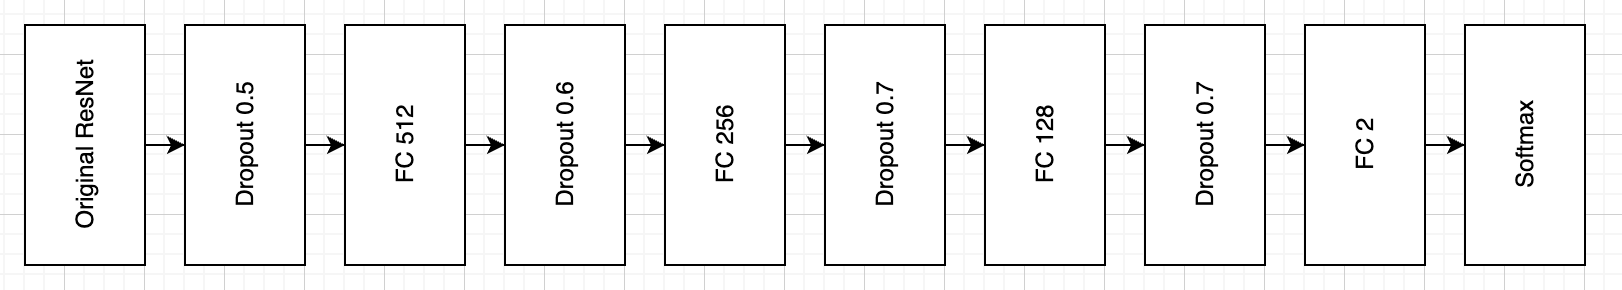
\includegraphics[width=\linewidth]{Materials/Methods/Mod2DResNet}
	\caption{Modified 2D ResNet model used for separation point predictions. The modifications lies in the added fully connected layers after the original fully connected layer of size 1000, and the added dropout layers.}
	\label{2DResNet}
\end{figure}

\subsection{Post-processing}
After using the 2D ResNet model to get segmentation predictions of each endoscopy video, the following post-processing approaches were used to translate them into concrete separation predictions.

\subsubsection{Random Walker approach}
Random Walker is an image segmentation algorithm which has a walker move around an image. Several seed points with an annotated label are spread across the image at initialization, and when the walker reaches a seed point, the pixel it started from will then be annotated with the corresponding label. The transition probabilities between pixels are based on the pixels' similarity, that is, if two pixels have the same intensity a transition to that pixel is likely. In an iterative algorithm, several walkers are simulated and the pixel will be annotated the class it reached the most times. Other ways to simulate the algorithm exists, an example would be to solve an anisotropic diffusion equation.\\
The Random Walker approach uses \textit{skimage.segmentatio.random\_walker} to make the noisy output from the segmentation more structured. As the skimage function expects an image the predicted segmentation is stacked on top of itself. This makes a 'up or down' transition for the Random Walker likely, but we are only interested in whether the Random Walker reaches the left or right 'end' where the seed points for a healthy and inflamed classification resides, and because the 'left/right' transition probabilities remain the same, this approach will yield the correct result. After applying the Random Walker approach we expect the new video segmentation to contain larger and more continuous blocks and ideally only two blocks giving us the predicted separation point. 

\subsubsection{Scoring heuristic}
The scoring heuristic scores each 'transition' between the segmentations of a video based on the confidence of the predictions. For each frame, the confidence of that prediction (the output probability for the most likely class) is multiplied by the confidence of the frame immediately to the right. This gives a score between 0.25 and 1.0 to each 'transition' between the frames. This gives a high score if the model is confident in its prediction of two frames next to each other, but a low score if it is insecure. When each transition have been scored, the separation point is chosen as the point with the lowest score. If several transitions share a lowest score, the median is taken to choose a separation point which actually have a lowest score, rather than likely choosing a random point by using the mean.

\subsection{Treatment prediction}\label{treatmentprediction}
When doing treatment predictions we have a total of five classes as four different treatments were prescribed to the patients in the datasets, along with some patients being healthy. The treatment prescribed is highly correlated with how much of the colon and which parts of the colon is experiencing inflammation. When doing segmentations of the videos, this is essentially the information we get, and it is thus attempted to predict the treatment from these segmentations. This means, based on a video segmentation we will predict which of the five classes of treatment the patient received.\\
To obtain the desired video segmentations, the best performing 2D ResNet model is used on each of the 30 suitable videos for this task. This would ideally give us one continuous block of inflammation predictions followed by one continuous block of healthy predictions for each video, which would be similar to what a doctor would observe. Because the videos vary in lengths, a vector consisting of 1000 evenly spaced samples is made from each of the 30 segmentations. These 30 vectors of size 1000 are then used to predict on.\\
For this task a 1D ResNet is used to process the vectors. Modifications are made similar to the 2D ResNet previously used, and can be seen in \autoref{1DResNet}. 'One-vs-rest' binary classifiers were also trained to make ROC curves. For these models the last fully connected layer reducing the feature size to 5 was replaced with a fully connected layer reducing the feature size to 1 and the softmax activation function was replaced with a sigmoid activation function.

\begin{figure}[H]
	\centering
	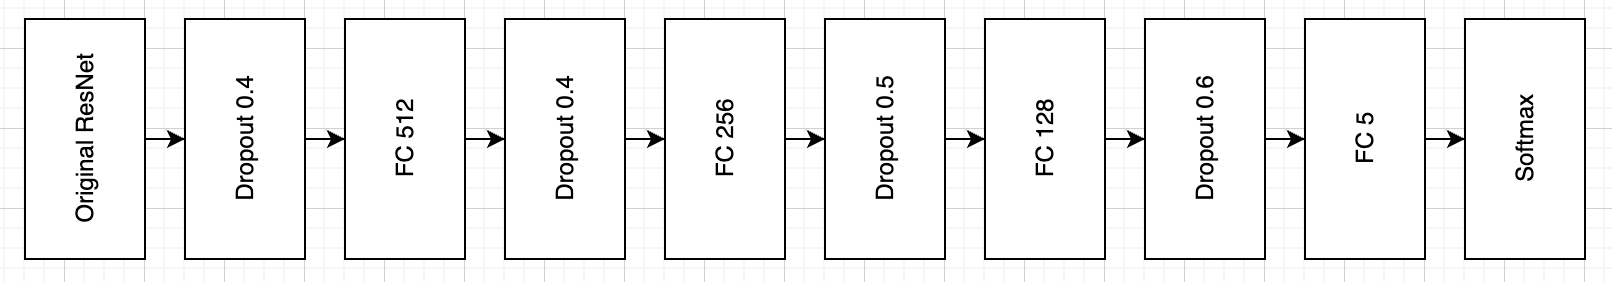
\includegraphics[width=\linewidth]{Materials/Methods/Mod1DResNet}
	\caption{Modified 1D ResNet model used for treatment predictions. The modifications lies in the added fully connected layers after the original fully connected layer of size 1000, and the added dropout layers.}
	\label{1DResNet}
\end{figure}

\subsection{U-Net for video segmentation}
As another approach to get video segmentations for the treatment classification, a 1D U-Net was used to predict the video segmentations. This approach was used to reduce the noise of the 2D ResNet predictions and thus to provide more accurate video segmentation vectors for treatment predictions.\\ 
The segmentation results of the 2D ResNet was used as input for the 1D U-Net model and the true segmentation was used as target vectors. Given the videos vary in length a vector consisting of 1000 evenly spaced samples is made from the results of the 2D ResNet and the target vector.

\subsection{U-Net predictions for treatment prediction}
With the refined U-Net segmentations, treatment predictions were then again attempted using the same approach as previously presented, but now using the U-Net segmentations as input. The same 1D ResNet models from \autoref{treatmentprediction} were used again.
	